%%%%%%%%%%%%%%%%%%%%%%%%%%%%%%%%%%%%%%%%%
% Structured General Purpose Assignment
% LaTeX Template
%
% This template has been downloaded from:
% http://www.latextemplates.com
%
% Original author:
% Ted Pavlic (http://www.tedpavlic.com)
%
% Note:
% The \lipsum[#] commands throughout this template generate dummy text
% to fill the template out. These commands should all be removed when 
% writing assignment content.
%
%%%%%%%%%%%%%%%%%%%%%%%%%%%%%%%%%%%%%%%%%

%----------------------------------------------------------------------------------------
%	PACKAGES AND OTHER DOCUMENT CONFIGURATIONS
%----------------------------------------------------------------------------------------
\documentclass{Askarticle}
\usepackage[utf8]{inputenc}
\usepackage{fancyhdr} % Required for custom headers
\usepackage{lastpage} % Required to determine the last page for the footer
\usepackage{extramarks} % Required for headers and footers
\usepackage{graphicx} % Required to insert images
\usepackage{lipsum} % Used for inserting dummy 'Lorem ipsum' text into the template
\usepackage{amsmath}
\usepackage{amsfonts}
\usepackage{listings}
\usepackage{color}
%\usepackage{slashbox}
\usepackage{verbatim}
\usepackage{graphicx}

\usepackage{fancybox}
\usepackage{tikz}

 \usepackage[utf8]{inputenc}
\usepackage[english]{babel}
 
\usepackage{amsthm}
 
\usepackage[colorinlistoftodos]{todonotes}
\usepackage{algorithm}
\usepackage{algpseudocode}

\usepackage{color} %for colored boxes
\usepackage{empheq}

\usepackage{listings} %to include Code
\usepackage{booktabs} %for tables



\usepackage{geometry}
 \geometry{
 a4paper,
 total={210mm,297mm},
 left=20mm,
 right=20mm,
 top=20mm,
 bottom=20mm,
 }

%---------------------------------------------------------------------------------------------
%LISTINGS INITIAL
%---------------------------------------------------------------------------------------------
\definecolor{codegreen}{rgb}{0,0.6,0}
\definecolor{codegray}{rgb}{0.5,0.5,0.5}
\definecolor{codepurple}{rgb}{0.58,0,0.82}
\definecolor{backcolour}{rgb}{0.95,0.95,0.92}
 
\lstdefinestyle{mystyle}{
    backgroundcolor=\color{backcolour},   
    commentstyle=\color{codegreen},
    keywordstyle=\color{magenta},
    numberstyle=\tiny\color{codegray},
    stringstyle=\color{codepurple},
    basicstyle={\ttfamily \footnotesize},
    breakatwhitespace=false,         
    breaklines=true,                 
    captionpos=b,                    
    keepspaces=true,                 
    numbers=left,                    
    numbersep=5pt,                  
    showspaces=false,                
    showstringspaces=false,
    showtabs=false,                  
    tabsize=2
}
 
\lstset{style=mystyle}
%---------------------------------------------------------------------------------------------
% Margins
\topmargin=-0.45in
\evensidemargin=0in
\oddsidemargin=0in
\textwidth=6.5in
\textheight=9.0in
\headsep=0.25in 

\linespread{1.1} % Line spacing

% Set up the header and footer
\pagestyle{fancy}
%\lhead{\hmwkAuthorName} % Top left header
\rhead{\hmwkClass\ : \hmwkTitle} % Top center header
%\chead{\firstxmark} % Top right header
\lfoot{\lastxmark} % Bottom left footer
\cfoot{} % Bottom center footer
\rfoot{Page\ \thepage\ of\ \pageref{LastPage}} % Bottom right footer
\renewcommand\headrulewidth{0.4pt} % Size of the header rule
\renewcommand\footrulewidth{0.4pt} % Size of the footer rule

\setlength\parindent{0pt} % Removes all indentation from paragraphs

%----------------------------------------------------------------------------------------
%	DOCUMENT STRUCTURE COMMANDS
%	Skip this unless you know what you're doing
%----------------------------------------------------------------------------------------

% Header and footer for when a page split occurs within a problem environment
\newcommand{\enterProblemHeader}[1]{
\nobreak\extramarks{#1}{#1 continued on next page\ldots}\nobreak
\nobreak\extramarks{#1 (continued)}{#1 continued on next page\ldots}\nobreak
}

% Header and footer for when a page split occurs between problem environments
\newcommand{\exitProblemHeader}[1]{
\nobreak\extramarks{#1 (continued)}{#1 continued on next page\ldots}\nobreak
\nobreak\extramarks{#1}{}\nobreak
}

\setcounter{secnumdepth}{0} % Removes default section numbers
\newcounter{homeworkProblemCounter} % Creates a counter to keep track of the number of problems

\newcommand{\homeworkProblemName}{}
\newenvironment{homeworkProblem}[1][Problem \arabic{homeworkProblemCounter}]{ % Makes a new environment called homeworkProblem which takes 1 argument (custom name) but the default is "Problem #"
\stepcounter{homeworkProblemCounter} % Increase counter for number of problems
\renewcommand{\homeworkProblemName}{#1} % Assign \homeworkProblemName the name of the problem
\section{\homeworkProblemName} % Make a section in the document with the custom problem count
\enterProblemHeader{\homeworkProblemName} % Header and footer within the environment
}{
\exitProblemHeader{\homeworkProblemName} % Header and footer after the environment
}

\newcommand{\problemAnswer}[1]{ % Defines the problem answer command with the content as the only argument
\noindent\framebox[\columnwidth][c]{\begin{minipage}{0.98\columnwidth}#1\end{minipage}} % Makes the box around the problem answer and puts the content inside
}

\newcommand{\homeworkSectionName}{}
\newenvironment{homeworkSection}[1]{ % New environment for sections within homework problems, takes 1 argument - the name of the section
\renewcommand{\homeworkSectionName}{#1} % Assign \homeworkSectionName to the name of the section from the environment argument
\subsection{\homeworkSectionName} % Make a subsection with the custom name of the subsection
\enterProblemHeader{\homeworkProblemName\ [\homeworkSectionName]} % Header and footer within the environment
}{
\enterProblemHeader{\homeworkProblemName} % Header and footer after the environment
}
   
%----------------------------------------------------------------------------------------
%	NAME AND CLASS SECTION
%----------------------------------------------------------------------------------------
\newcommand\given[1][]{\:#1\vert\:} %define new command
\newcommand{\hmwkTitle}{Midterm} % Assignment title
\newcommand{\hmwkDueDate}{\today} % Due date
\newcommand{\hmwkClass}{TIM\ 245 - Data Mining} % Course/class
\newcommand{\hmwkClassTime}{4:20pm} % Class/lecture time
\newcommand{\hmwkClassInstructor}{Instructor: Tyler Munger} % Teacher/lecturer
\newcommand{\hmwkAuthorNameB}{Panos Karagiannis}
\newcommand{\hmwkOption}{Homework Heavy Option}
\newcommand{\hmwkIDA}{ID: -}

\newcommand{\Prb}{\mathbb{P}}
\newcommand{\N}{\mathcal{N}}
\newcommand{\R}{\mathbb{R}}
\newcommand{\E}{\mathbb{E}}
\newcommand{\answer}{\noindent\rule{16cm}{0.9pt}
		
		\large{\textbf{\underline{Answer:}}}

		\vspace{0.5cm}}
%----------------------------------------------------------------------------------------
%	TITLE PAGE
%----------------------------------------------------------------------------------------

\title{
\vspace{2in}
\textmd{\textbf{\hmwkClass:\ \hmwkTitle}}\\
\normalsize\vspace{0.1in}\small{Due:\ \textit{\hmwkDueDate}}\\
\vspace{0.1in}\large{\textit{\hmwkClassInstructor}}
\vspace{3in}
}

\author{\begin{tabular}{ l r }
					 \hmwkAuthorNameB \\
					\multicolumn{1}{c}{\hmwkIDA}
				\end{tabular}}
\date{} % Insert date here if you want it to appear below your name

%----------------------------------------------------------------------------------------

\begin{document}

\maketitle

%----------------------------------------------------------------------------------------
%	TABLE OF CONTENTS
%----------------------------------------------------------------------------------------

%\setcounter{tocdepth}{1} % Uncomment this line if you don't want subsections listed in the ToC

\newpage
\tableofcontents
\newpage

\newtheorem{theorem}{Theorem}
\newtheorem{panostheorem}{Theorem}
\newtheorem{claim}[theorem]{Claim}
\newtheorem{definition}[panostheorem]{Definition}

%----------------------------------------------------------------------------------------
%	BLUE BOX
%----------------------------------------------------------------------------------------



\definecolor{myblue}{rgb}{.8, .8, 1}



\newlength\mytemplen
\newsavebox\mytempbox

\makeatletter
\newcommand\mybluebox{%
    \@ifnextchar[%]
       {\@mybluebox}%
       {\@mybluebox[0pt]}}

\def\@mybluebox[#1]{%
    \@ifnextchar[%]
       {\@@mybluebox[#1]}%
       {\@@mybluebox[#1][0pt]}}

\def\@@mybluebox[#1][#2]#3{
    \sbox\mytempbox{#3}%
    \mytemplen\ht\mytempbox
    \advance\mytemplen #1\relax
    \ht\mytempbox\mytemplen
    \mytemplen\dp\mytempbox
    \advance\mytemplen #2\relax
    \dp\mytempbox\mytemplen
    \colorbox{myblue}{\hspace{1em}\usebox{\mytempbox}\hspace{1em}}}

\makeatother

%----------------------------------------------------------------------------------------
%	PROBLEM 1
%----------------------------------------------------------------------------------------

\begin{homeworkProblem}[Problem \arabic{homeworkProblemCounter}: Exploratory Data Analysis and Data Cleaning (50 points)  ]
The product management team has heard that data quality can be a significant issue when trying to create a good predictive model. Therefore, they have asked you to first assess the collected data and determine if it is suitable for creating an employee satisfaction prediction model.



\begin{enumerate}
\item Before you start, the product management team would like a written statement of your process, for Exploratory Data Analysis (EDA). (Hint: The process might include the steps such as compute descriptive statistics or determine threshold for outliers)
\item 	Then, they would like you to apply your EDA process to the collected data-set and format the results into a well-structured report.
\item 	Lastly, they would like you to provide them with a set of recommended data pre-processing steps (cleaning, transformation, etc.) for addressing any data quality issues that were discovered during the EDA process.
\end{enumerate}


%In addition, we will explore whether the dataset contains any \textbf{missing values} and we will also suggest a way of \textbf{handling them}.
%We define outliers to be data points that are significantly far from the central tendency and we adopt a Parametric Outlier Analysis where we select a quantile cutoff for outliers.
\noindent\rule{16cm}{0.9pt}
		
\large{\textbf{\underline{Answer:}}}

\begin{enumerate}
\item Real world data are often \textbf{Incomplete}, \textbf{Noisy} as well as \textbf{Inconsistent}. Our Exploratory Data Analysis will consist of a combination of \textbf{visual} and \textbf{quantitative} tools to answer important questions for each selected attribute in our dataset. More precisely, for each attribute we will look into descriptive statistics such as the \textbf{typical value}, the \textbf{spread} for a typical value and whether it affects other attributes (\textbf{correlation}). Moreover, we will employ visual tools in order to estimate a good distributional fit for the data but also determine the existence of outliers (\textbf{histogram, box plots}). Also, we will use a combination of visual tools and descriptive statistics (\textbf{scatter plot, correlation}) to determine the co-linearity of attributes. Finally, we \textbf{omit} the attribute \texttt{id} since it simply functions as a unique identifier and hence no meaningful insights can be extracted.


\begin{table}[H]
\caption{Pearson Correlation Matrix for all attributes}
\centering
\begin{tabular}{lrrrrrrrr}
\hline\hline
{} &        id &  current\_sat &  last\_eval\_sat &  n\_proj &  m\_hours &  time &  promotion &    salary \\
\midrule
id                                 &  1.000000 &                    0.019087 &                            0.004644 &        -0.003514 &              0.003326 &               0.004154 &                  -0.000580 &  0.020131 \\
current\_sat         &  0.019087 &                    1.000000 &                            0.105021 &        -0.142970 &             -0.020048 &              -0.100866 &                   0.025605 &  0.047476 \\
last\_eval\_sat &  0.004644 &                    0.105021 &                            1.000000 &         0.349333 &              0.339742 &               0.131591 &                  -0.008684 & -0.014793 \\
n\_proj                    & -0.003514 &                   -0.142970 &                            0.349333 &         1.000000 &              0.417211 &               0.196786 &                  -0.006064 & -0.004628 \\
m\_hours               &  0.003326 &                   -0.020048 &                            0.339742 &         0.417211 &              1.000000 &               0.127755 &                  -0.003544 & -0.004719 \\
time              &  0.004154 &                   -0.100866 &                            0.131591 &         0.196786 &              0.127755 &               1.000000 &                   0.067433 &  0.044233 \\
promotion         & -0.000580 &                    0.025605 &                           -0.008684 &        -0.006064 &             -0.003544 &               0.067433 &                   1.000000 &  0.091139 \\
salary                             &  0.020131 &                    0.047476 &                           -0.014793 &        -0.004628 &             -0.004719 &               0.044233 &                   0.091139 &  1.000000 \\
\hline
\end{tabular}
\label{table:corr}
\end{table}

\newpage
\item Therefore for each attribute we discover the following information:\\
\texttt{current\_satisfaction\_score}: 
\begin{enumerate}
\item \textsc{Typical Value}: Calculating the mean for this attribute we get that the average score is $61.28$
\item \textsc{Spread}: The standard deviation (sample) for this data is $24.86$. Since significant outliers exist in this attribute a better measure of dispersion is $mad=19$
\item \textsc{ Distributional fit}: Drawing a histogram of the data we see that the distribution looks slightly skewed to the left (i.e. few employees have low satisfaction score)
\item  \textsc{Correlation}: Referring to $Table 1$ we see that \texttt{current\_satisfaction\_score} is most strongly positively correlated with  \texttt{last\_evalualtion\_satisfaction\_score}, whereas, it is most strongly negatively correlated with \texttt{number\_projects}. 
\item 	\textsc{Outliers}: There exist some outliers which is evident from the magnitude of the measures of dispersion ($sd=24.86$, $mad=19$).
\end{enumerate}

\begin{figure}[htp]
\centering
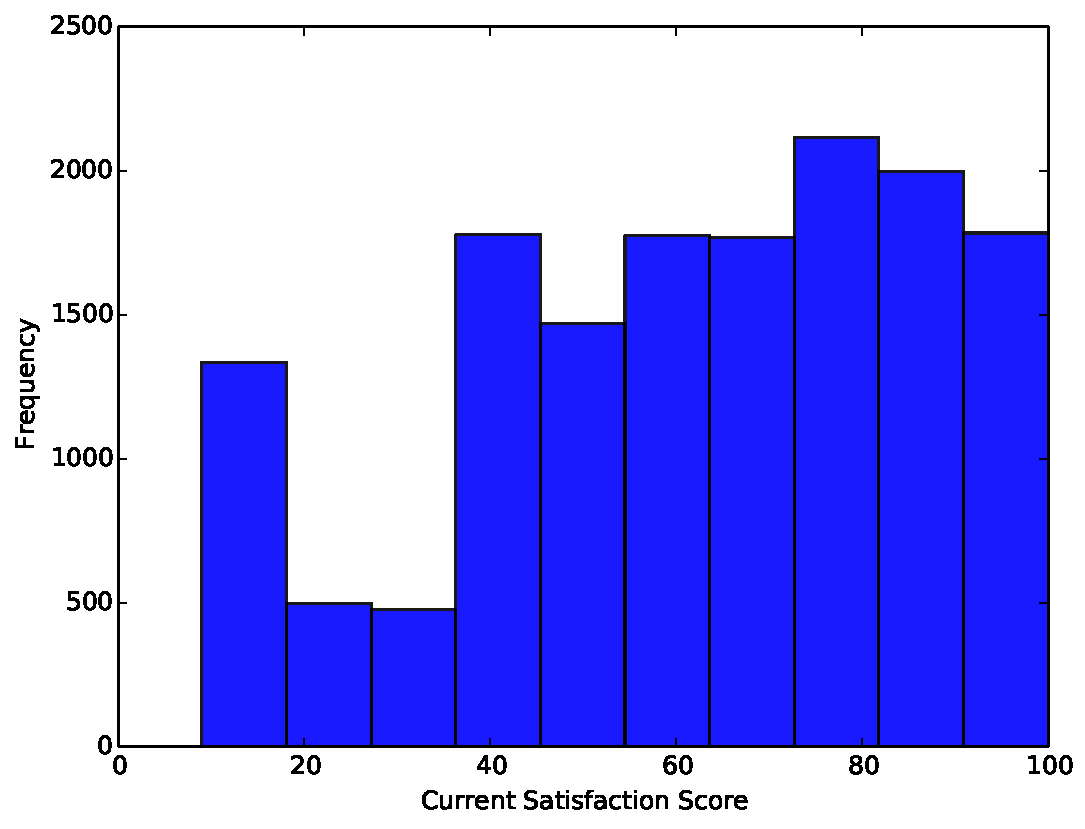
\includegraphics[width=.5\textwidth]{../Code/Plots/curr_hist.pdf}\hfill
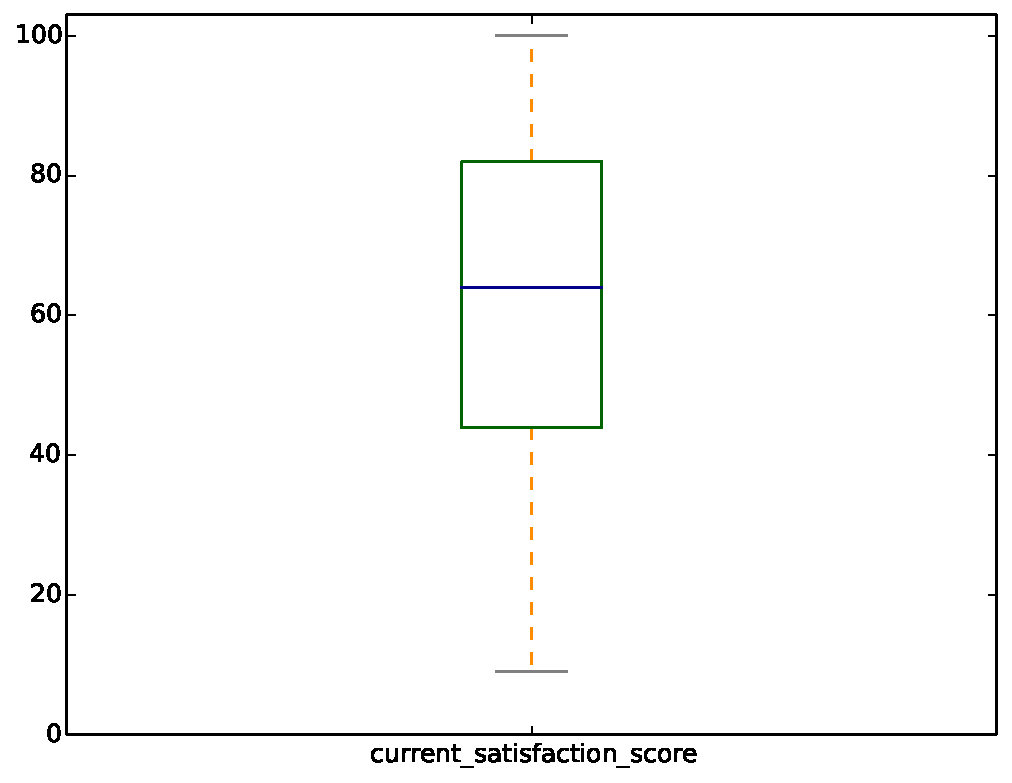
\includegraphics[width=.5\textwidth]{../Code/Plots/curr_box.pdf}\hfill
\caption{Histograms and Box Plot for \texttt{current\_satisfaction\_score}}
\label{fig:figure3}
\end{figure}

\texttt{last\_evalualtion\_satisfaction\_score}: 
\begin{enumerate}
\item \textsc{Typical Value}: Calculating the mean for this data the average score is approximately $71.61$
\item \textsc{Spread}: The standard deviation (sample) for this data is $17.11$ and the $mad=15$.

\item \textsc{distributional fit}: Drawing a histogram of the data we see that the distribution looks to be relatively symmetric and centered around the mean, even though a few outliers exist with very small \texttt{last\_evalualtion\_satisfaction\_score}.

\item  \textsc{Correlation}: Referring to $Table 1$ we see that \texttt{last\_evalualtion\_satisfaction\_score} is most strongly positively correlated with  \texttt{current\_satisfaction\_score}, whereas, it is most strongly negatively correlated with \texttt{salary}. 

\item \textsc{Outliers}: Looking at the histogram as well as at the standard deviation there does not seem to be significant outliers for this attribute. Here we don't need to look at the $mad$ measure since our data are relatively symmetric around the mean.
\end{enumerate}

\begin{figure}[htp]
\centering
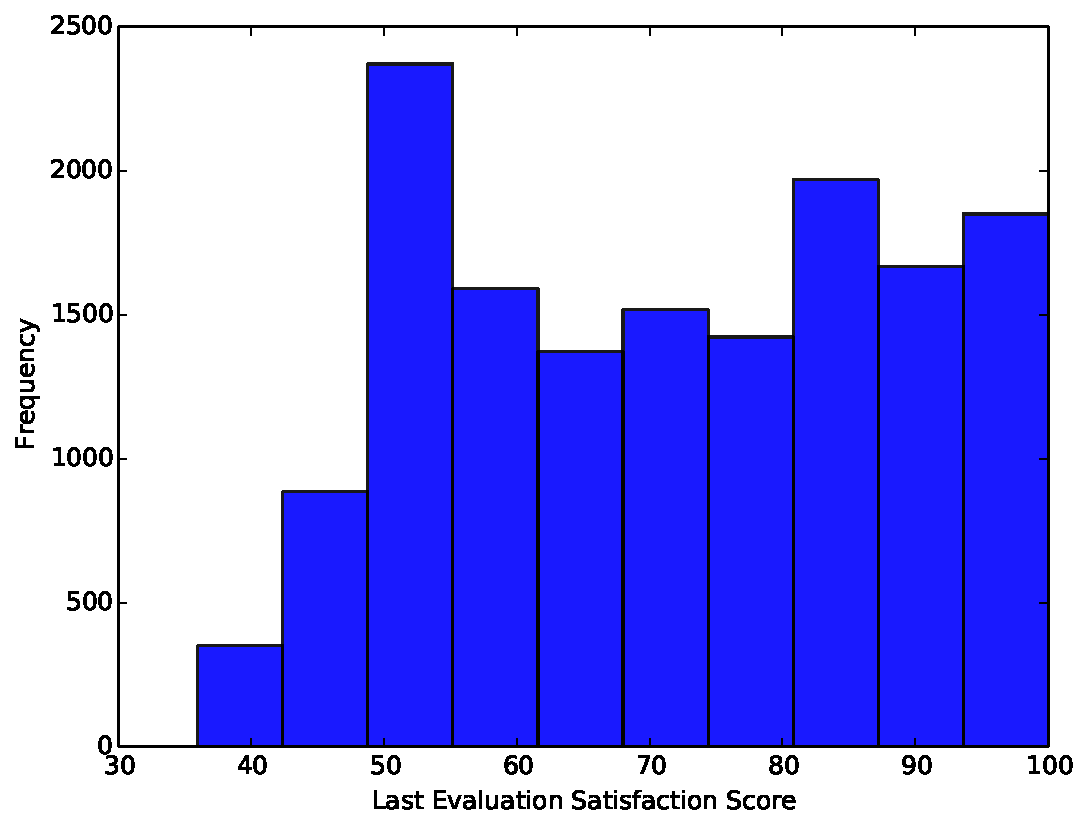
\includegraphics[width=.5\textwidth]{../Code/Plots/last_hist.pdf}\hfill
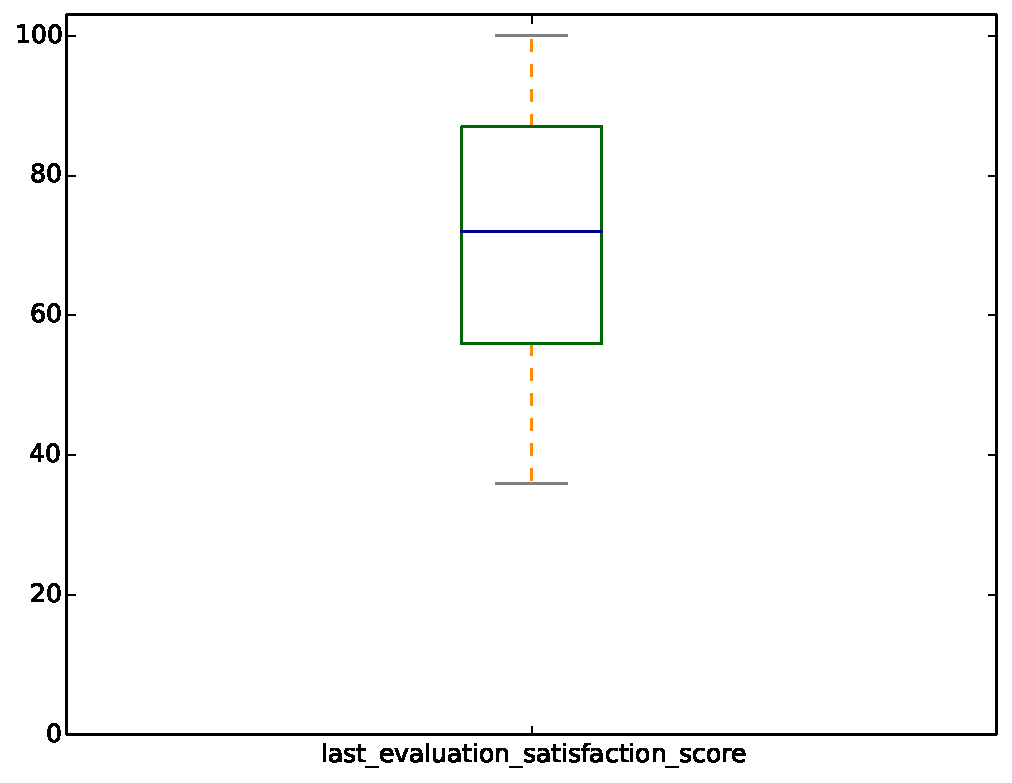
\includegraphics[width=.5\textwidth]{../Code/Plots/last_box.pdf}\hfill
\caption{Histograms and Box Plot for \texttt{last\_evalualtion\_satisfaction\_score}}
\label{fig:figure3}
\end{figure}

\texttt{number\_projects}: 
\begin{enumerate}
\item \textsc{Typical Value}: Calculating the mean for this data we get that the average budget is approximately $3.80$

\item \textsc{Spread}: The standard deviation (sample) for this data is $1.23$. Since significant outliers exist in this attribute a better measure of dispersion is $mad=1$.

\item \textsc{Distributional fit}: Drawing a histogram of the data we see that the distribution looks to be symmetric around the mean with a few outliers

\item  \textsc{Correlation}: From $Table 1$ we see that this attribute is most strongly positively correlated with  \texttt{average\_monthly\_hours}, whereas, it is most strongly negatively correlated with \texttt{current\_satisfaction\_score}. 

\item \textsc{Outliers}: As before, looking at the histogram as well as at the standard deviation there does not seem to be significant outliers for this attribute. Here we don't need to look at the $mad$ measure since our data are relatively symmetric around the mean.
\end{enumerate}

\begin{figure}[htp]
\centering
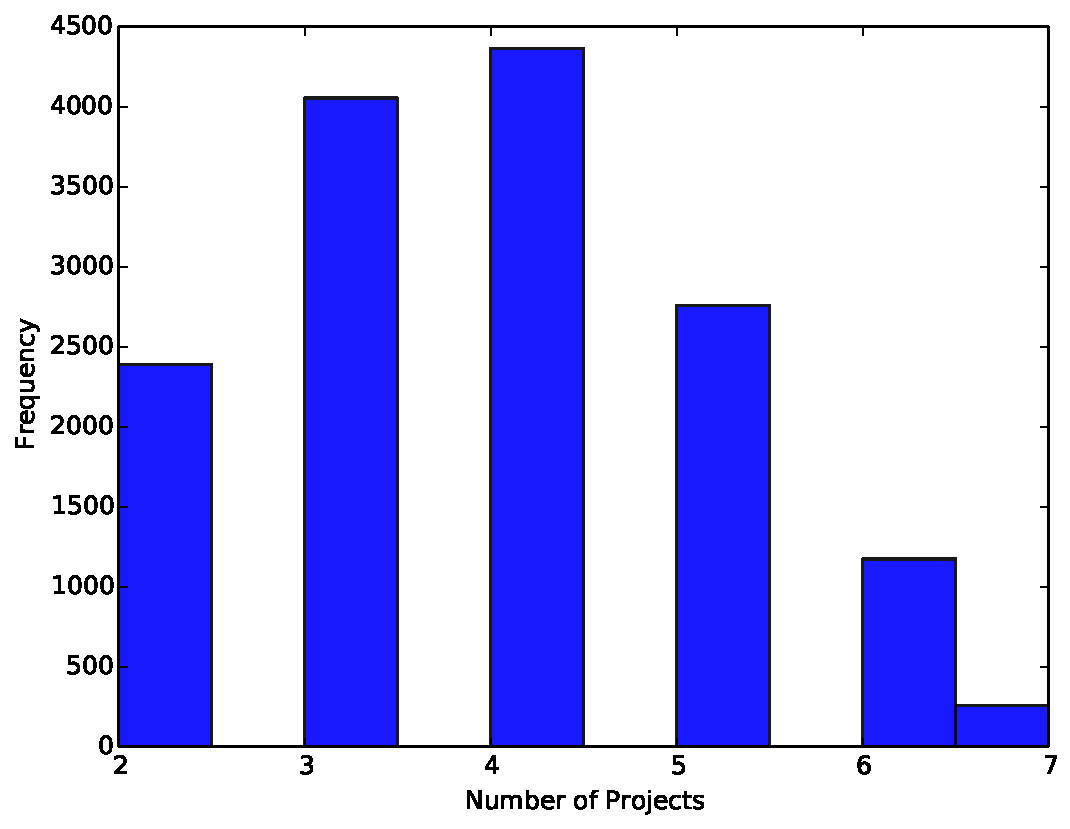
\includegraphics[width=.5\textwidth]{../Code/Plots/proj_hist.pdf}\hfill
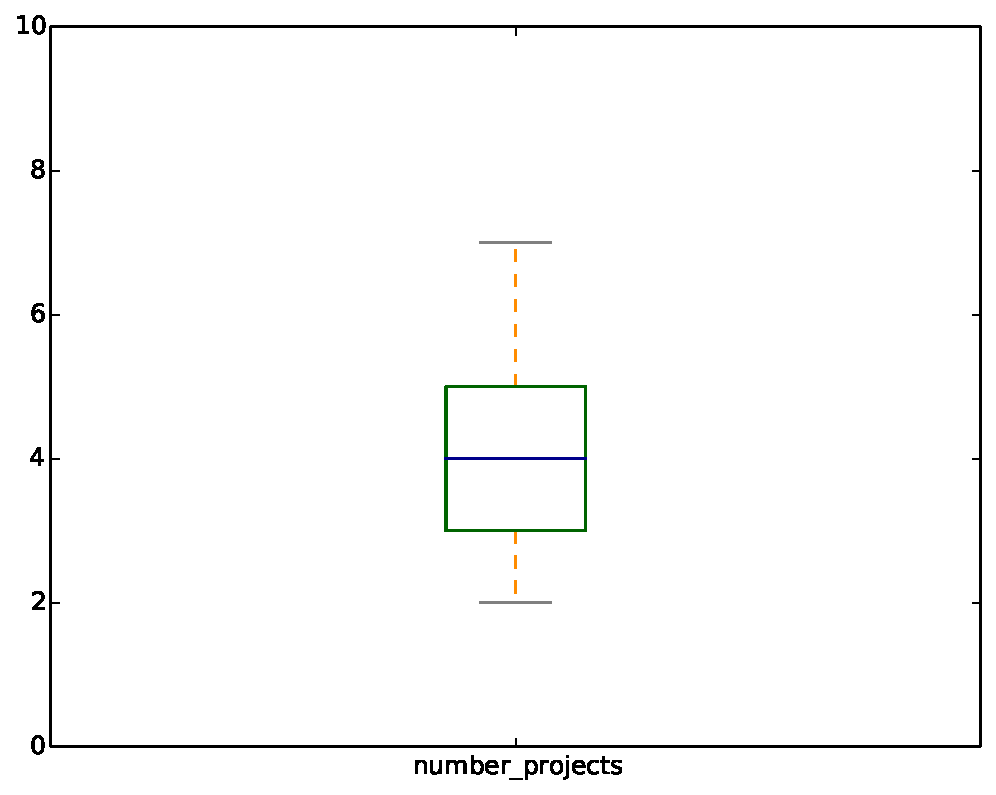
\includegraphics[width=.5\textwidth]{../Code/Plots/proj_box.pdf}\hfill
\caption{Histograms and Box Plot for \texttt{number\_projects}}
\label{fig:figure3}
\end{figure}

\texttt{average\_monthly\_hours}: 
\begin{enumerate}
\item \textsc{Typical Value}: Calculating the mean for this data we get that the average budget is approximately $201.05$

\item \textsc{Spread}: The standard deviation (sample) for this data is $49.94$. Since significant outliers exist in this attribute a better measure of dispersion is $mad=44$.

\item \textsc{Distributional fit}: Drawing a histogram of the data we see that the distribution looks to be symmetric around the mean with a few outliers

\item  \textsc{Correlation}: From $Table 1$ we see that this attribute is most strongly positively correlated with  \texttt{time\_spent\_at\_company}, whereas, it is most strongly negatively correlated with \texttt{current\_satisfaction\_score}. 

\item \textsc{Outliers}: As before, looking at the histogram as well as at the standard deviation there does not seem to be significant outliers for this attribute. Here we don't need to look at the $mad$ measure since our data are relatively symmetric around the mean.
\end{enumerate}

\begin{figure}[htp]
\centering
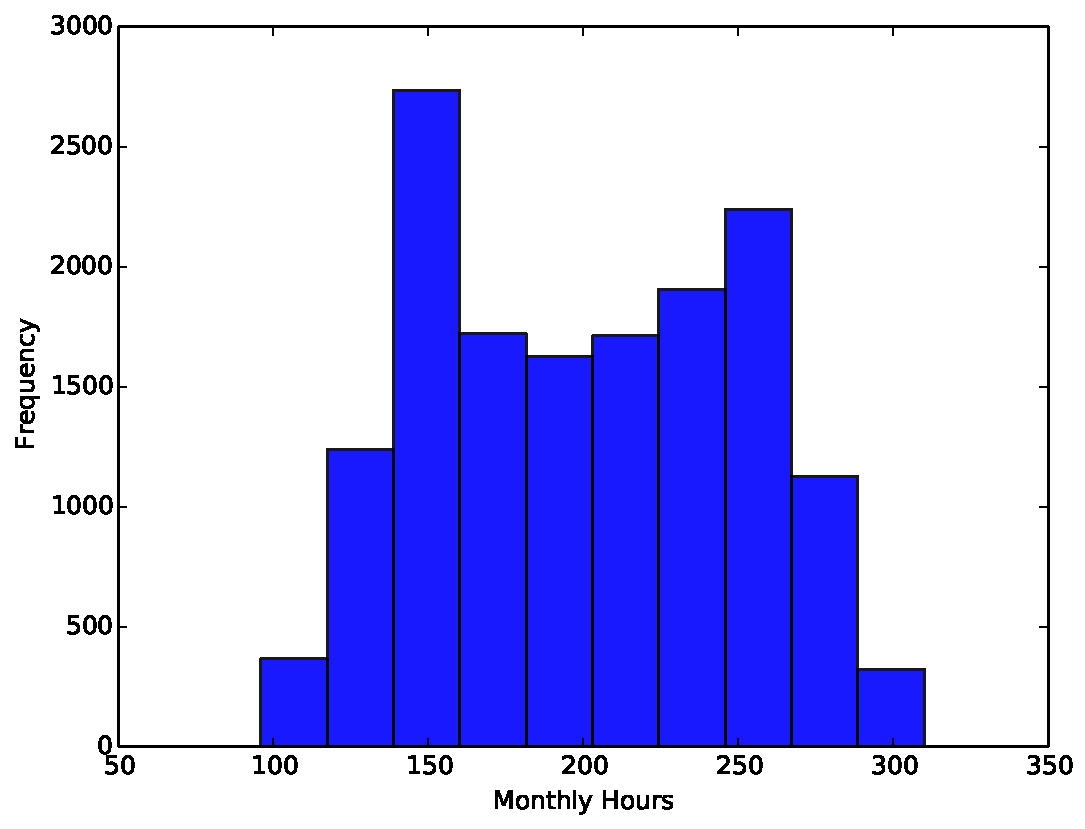
\includegraphics[width=.5\textwidth]{../Code/Plots/hours_hist.pdf}\hfill
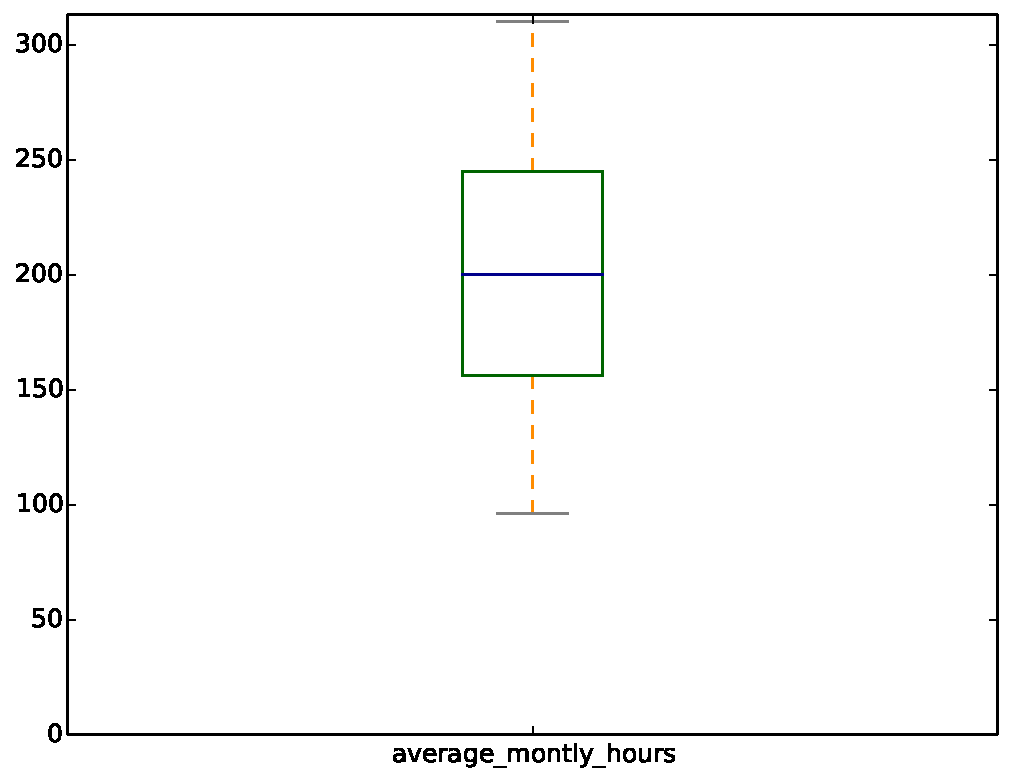
\includegraphics[width=.5\textwidth]{../Code/Plots/hours_box.pdf}\hfill
\caption{Histograms and Box Plot for \texttt{average\_monthly\_hours}}
\label{fig:figure3}
\end{figure}


\texttt{time\_spent\_at\_company}: 
\begin{enumerate}
\item \textsc{Typical Value}: Calculating the mean for this data we get that the average time spent is approximately $3.49$

\item \textsc{Spread}: The standard deviation (sample) for this data is $1.46$. Since outliers exist in this attribute another measure of dispersion is $mad=1$.

\item \textsc{Distributional fit}: Drawing a histogram of the data we see that the distribution is skewed to the right.
\item  \textsc{Correlation}: From $Table 1$ we see that this attribute is most strongly positively correlated with  \texttt{number\_projects}, whereas, it is most strongly negatively correlated with \texttt{current\_satisfaction\_score}. 

\item \textsc{Outliers}: Looking at the histogram, as well as, at the standard deviation there seem to be some outliers for this attribute. In particular there are a few datapoints with large \texttt{time\_spent\_at\_company}
 \end{enumerate}

\begin{figure}[htp]
\centering
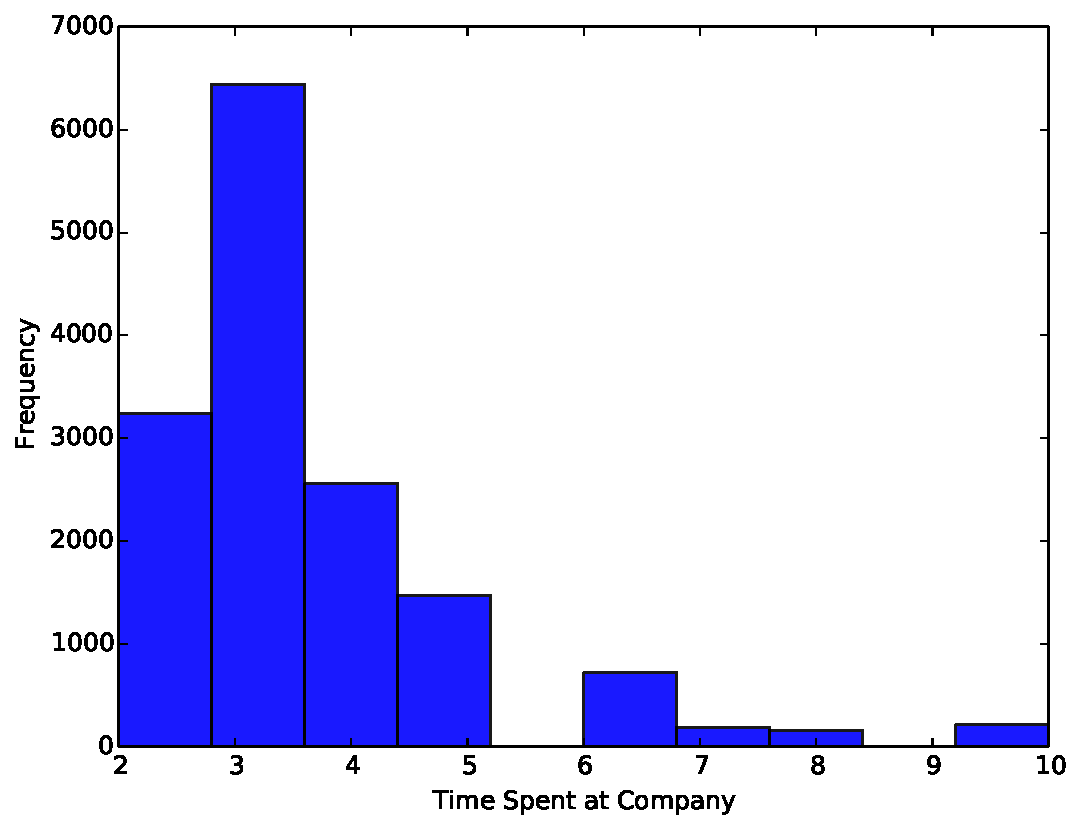
\includegraphics[width=.5\textwidth]{../Code/Plots/time_hist.pdf}\hfill
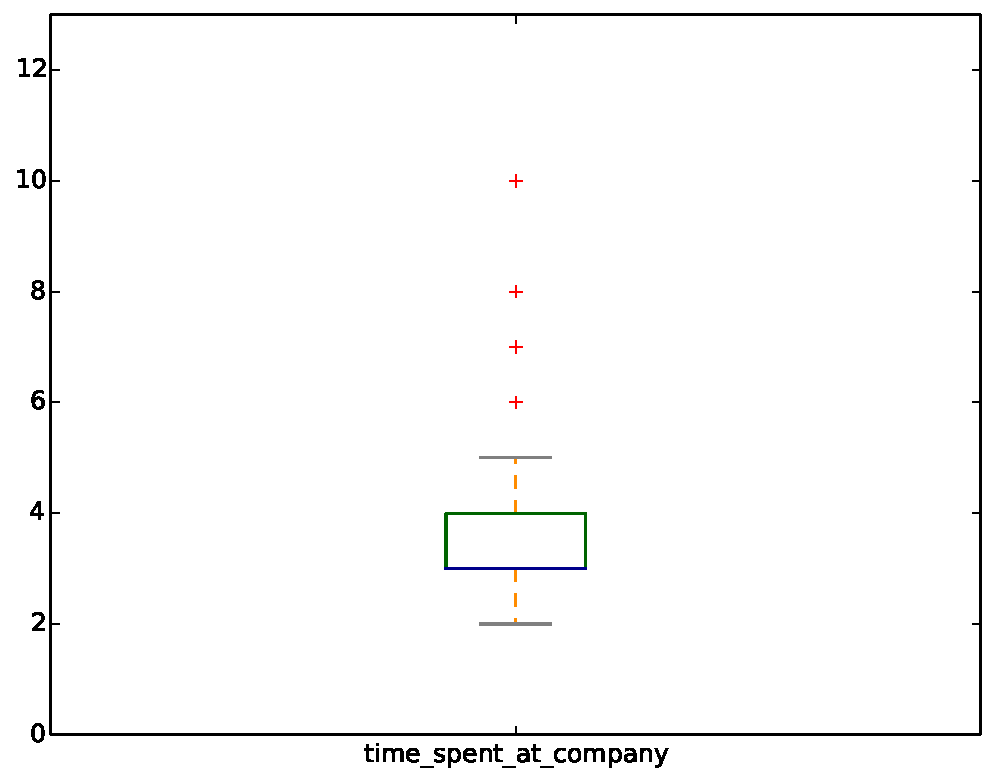
\includegraphics[width=.5\textwidth]{../Code/Plots/time_box.pdf}\hfill
\caption{Histograms and Box Plot for \texttt{time\_spent\_at\_company}}
\label{fig:figure3}
\end{figure}

\texttt{promotion\_in\_last\_5\_years}: 
\begin{enumerate}
\item \textsc{Typical Value}: Calculating the mean for this data we get that the average time spent is approximately $0.02$

\item \textsc{Spread}: The standard deviation (sample) for this data is $0.14$. 

\item \textsc{Distributional fit}: Drawing a histogram of the data we see the majority of the data is clustered in one bin.

\item  \textsc{Correlation}: From $Table 1$ we see that this attribute is not strongly correlated with any other attributes. 

\item \textsc{Outliers}: Looking at the histogram, as well as, at the standard deviation there seem to be very few datapoints that are not clustered in the bin $[0,1]$. \textbf{Therefore a box plot is omitted}. 
\end{enumerate}

\begin{figure}[htp]
\centering
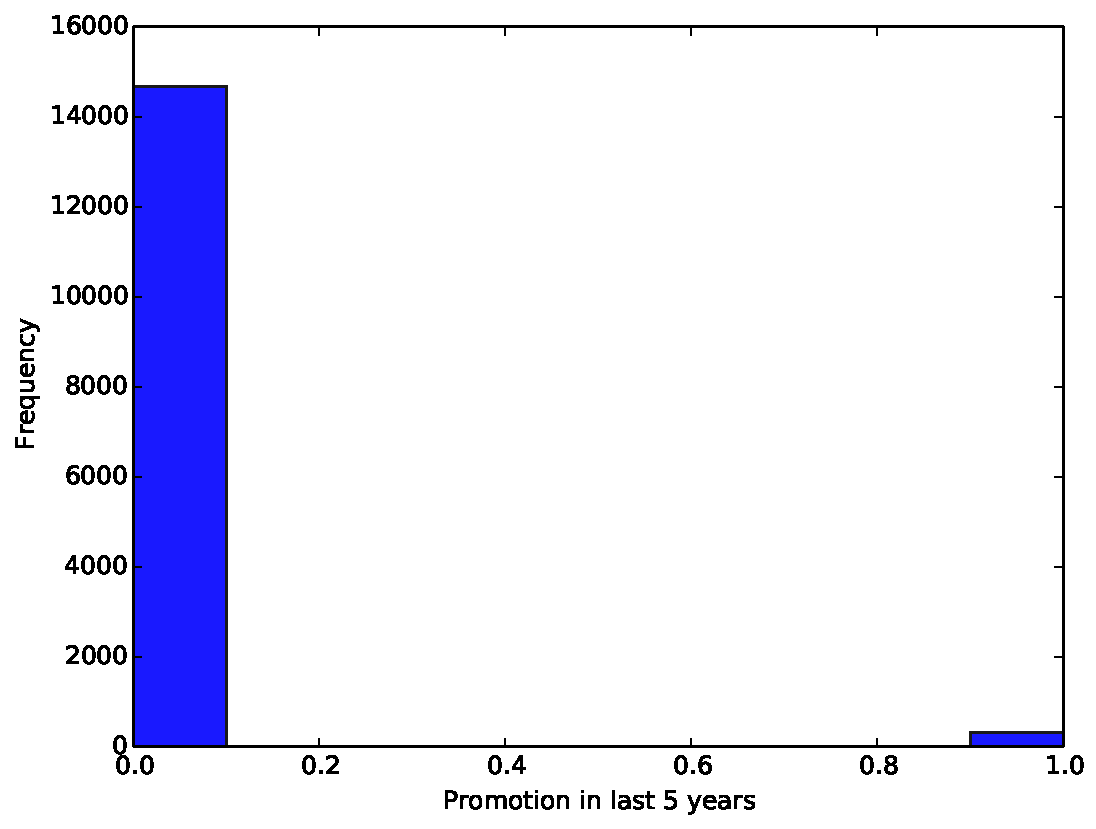
\includegraphics[width=0.5\textwidth]{../Code/Plots/promo_hist.pdf}\hfill
\caption{Histograms and Box Plot for \texttt{promotion\_in\_last\_5\_years}}
\label{fig:figure3}
\end{figure}


\texttt{salary}: 
\begin{enumerate}
\item \textsc{Typical Value}: Calculating the mean for this data we get that the average time spent is approximately $99,214$

\item \textsc{Spread}: The standard deviation (sample) for this data is $41,504$. 

\item \textsc{Distributional fit}: Drawing a histogram of the data we see that the distribution is skewed to the right.

\item  \textsc{Correlation}: From $Table 1$ we see that this attribute is not mostly correlated with any other attributes. 

\item \textsc{Outliers}: Looking at the histogram, as well as, at the standard deviation there seem to be significant outliers for this attribute.

\begin{figure}[htp]
\centering
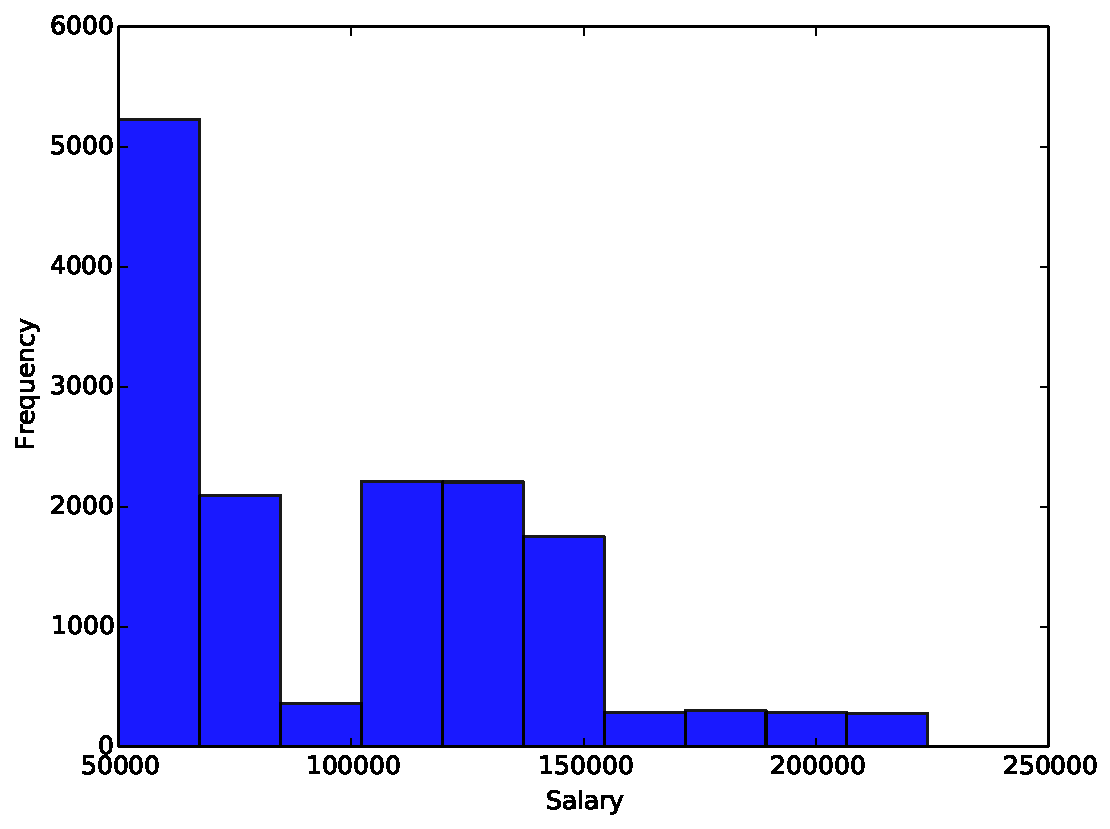
\includegraphics[width=0.5\textwidth]{../Code/Plots/salary_hist.pdf}\hfill
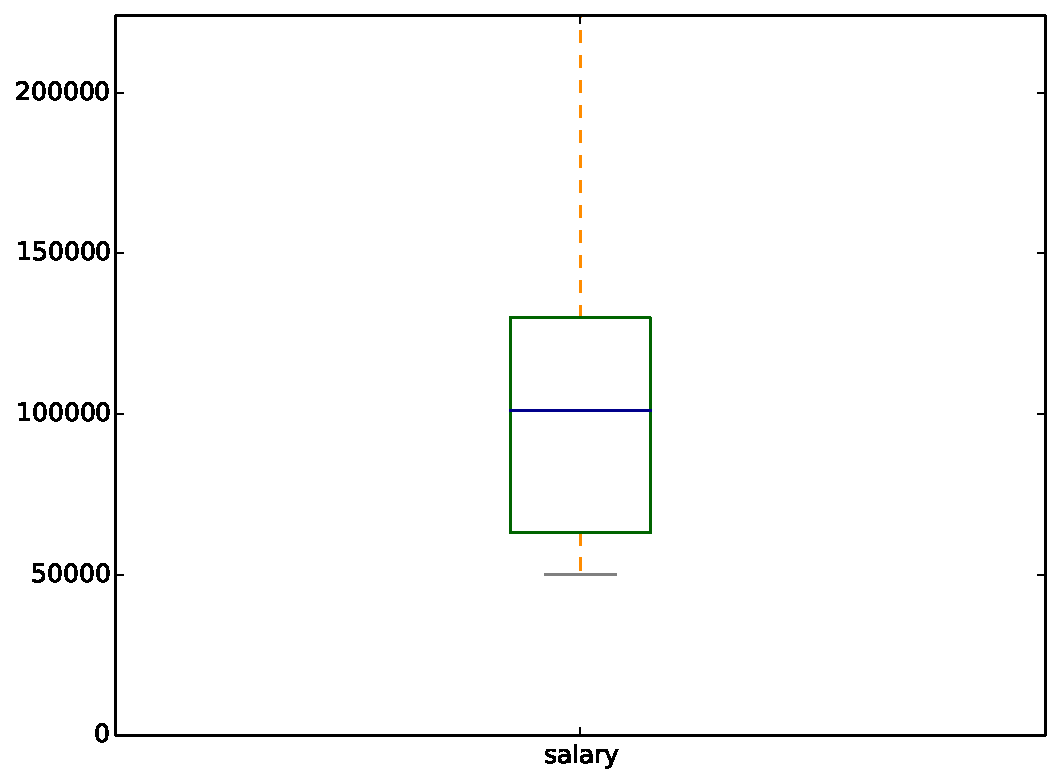
\includegraphics[width=0.5\textwidth]{../Code/Plots/salary_box.pdf}\hfill
\caption{Histograms and Box Plot for \texttt{salary}}
\label{fig:figure3}
\end{figure}
\end{enumerate}



\item One of the most important pre-processing steps, would be to locate and remove \textbf{duplicate and missing} values. Moreover, we need to \textbf{remove} \textbf{outlier} values from our attributes, since these values have a large impact on the quality of our results. Lastly, we could also
search for \textbf{inconsistencies} in the naming conventions of the \textbf{department} attribute.
% \textbf{normalize} our values in order to avoid one attribute dominating the value of the loss function.

\end{enumerate}

\end{homeworkProblem}
% To have just one problem per page, simply put a \clearpage after each problem
%----------------------------------------------------------------------------------------
%	PROBLEM 2
%----------------------------------------------------------------------------------------

\begin{homeworkProblem}[Problem \arabic{homeworkProblemCounter}: Predicting Employee Satisfaction (20 points) ]
The product management team has specified the requirement that the model is able to predict the employee's satisfaction score within +/- 25 points of the employee's actual score. You have been asked to perform the following tasks related to constructing the prediction model.

\begin{enumerate}
\item	First, apply your suggested data pre-processing from Problem 1 to the data-set and encode the nominal ``department'' attribute as a set of binary indicator attributes (dummy variables).
\item	Build and evaluate the following prediction models using the cleaned data-set: linear regression, ridge regression, lasso regression, and elastic net.
\item	Compare and contrast the performance of the different prediction models. Does your best model achieve the product managers' target accuracy? Do you think the model's performance is good? Explain why.
\item	What is the interpretation of the selected model? What can we say about the relationship between the input attributes and the satisfaction score?
\item	The product management team suggested including information about the manager of each employee into the model in order to improve accuracy. Do you think that this would help improve the model?s predictive accuracy? Explain why.
\end{enumerate}
	
\noindent\rule{16cm}{0.9pt}
		
\large{\textbf{\underline{Answer:}}}

\begin{enumerate}
\item First we need to explore whether our attributes contain duplicates. Assuming that each employee has a unique \texttt{id} then we can query for duplicate values of this attribute, to find that this dataset contains \textbf{no duplicate ids}. \\

Next performing a brute force search over all the entries of our dataset we determine that there are \textbf{no missing values}. \\


Based on our analysis in Question 1, we know that there exist \textbf{outliers} in our attributes. Therefore for all of our attributes we define $Q_{0}=5\%$ quantile and $Q_{1}=95\%$ quantile and then take the attributes which fall inside these quantiles. Following this process, we only keep the following values:

 \[  38 \leq \texttt{current\_satisfaction\_score} \leq 86 \]
  \[  53 \leq \texttt{last\_evaluation\_satisfaction\_score} \leq 90 \]
    \[  3 \leq \texttt{number\_projects} \leq 4 \]
    \[  148 \leq \texttt{average\_montly\_hours} \leq 255 \]
	\[  3 \leq \texttt{time\_spent\_at\_company} \leq 4 \]
	\[  0 \leq \texttt{promotion\_in\_last\_5\_years} \leq 1 \]
	\[  60,000 \leq \texttt{salary} \leq 137,000 \]

Finally, before converting our nominal value to numerical we \textbf{filter out inconsistencies}. Namely, we cluster:
\begin{itemize}
 \item \texttt{ \{r\&d , R\&D, rd, RandD\}} $\rightarrow$ \texttt{rd}
 \item  \texttt{\{Human\_Resources, human\_resources, hr\}} $\rightarrow$  \texttt{hr}
 \item  \texttt{\{product\_mng, product\_management\}} $\rightarrow$  \texttt{product\_mng }  
 \item  \texttt{\{IT,it, information\_technology \}} $\rightarrow$  \texttt{IT}
 \item  \texttt{\{sales, Sales\}} $\rightarrow$  \texttt{sales} 
 \item  \texttt{\{support, Support\}} $\rightarrow$  \texttt{support}
 \end{itemize}
%to prevent one attribute from dominating the ``sum'' in the \textbf{loss} function of the model then, we should use $z-score$ normalization to normalize every attribute based on its sum and standard deviation. \\

Next we attempt to encode the nominal variable ``department'' as a set of binary indicators. By processing our \texttt{csv} file, we notice that there are \textbf{in total $12$ distinct values} that this attribute takes. Therefore we encode these categories and hence we create $12$ \textbf{new binary numerical attributes}.

\item After discarding outliers we still have not merged the attributes together in order to create a single dataframe. We notice, that since we have deleted many values, ``merging'' the columns back together would result in having many \textbf{empty} cells. Therefore, we decide to delete all datapoints that contain at least $1$ empty cell. That reduces significantly our datasets's size from $14999$ instances to $2200$. \\

The \textbf{reason behind} deleting all instances with at least one empty cell, is that we do not want any outliers in our dataset. More precisely, if an empty cell exists, then it means that its original value had been filtered out by the procedure we followed in the previous step (step $1$), and hence, it was an outlier. An \textbf{alternative} approach would be to replace every missing value with the mean of that attribute, but that would inevitably distort the data and introduce some bias. This is not necessary here, since the resulting dataset size is adequate to allow our model to ``learn'' the weights and converge to a meaningful solution.\\

We split the cleaned data set into \emph{train} and \emph{test} in the ratio of $3:1$ and then we compute various linear models. We also compute the maximum and minimum difference in order to determine if a model can predict the employees satisfaction score within $25$ points. The results are summarized in the following table:

\begin{table}[H]
		\caption{MSE, Max/Min Difference for various linear models}
		\centering
		\begin{tabular}{c c c c}
		\hline\hline
		{} & MSE & Maximum Difference & Minimum Difference \\ [0.5ex] % inserts table %heading
		\hline
		Least Squares & 209.20 & 25.70 & -43.27 \\  
		Ridge&209.10 &25.06 & -48.67  \\
		
		Elastic Net  &208.92& 24.87  & -48.56  \\
		Lasso&208.80 & 24.70&-48.47  \\
		%\\ [1ex]
		\hline
		\end{tabular}\\[0.5cm]
		\label{table:nonlin}
\end{table}


\item We see that the simple linear  \emph{Least Squares} model has the largest $MSE$ which is logical since it does not penalize for the magnitude of the coefficients, as a result it is much more likely to overfit the data. \emph{Ridge Regression} performs better than \emph{Least Squares}, nevertheless, its $MSE$ score is worse than both  \emph{Elastic Net and Lasso}. It is worth mentioning, that when we compute the coefficients for  \emph{Ridge Regression} we get that none of them is $0$, thus verifying that \textbf{ridge regression does not perform variable selection.} On the contrary,  \emph{Lasso} is able to perform variable selection and therefore increase its accuracy achieving the smallest $MSE$ error among all other methods. Also,  \emph{Elastic Net} is a hybrid method that uses both \emph{Ridge and Lasso Regression} and manages to perform very similarly to \emph{Lasso}. Therefore, if I were to suggest any model to the management of the company I would recommend \textbf{Lasso}, because it has the smallest $MSE$. \\

\begin{figure}[htp]
\centering
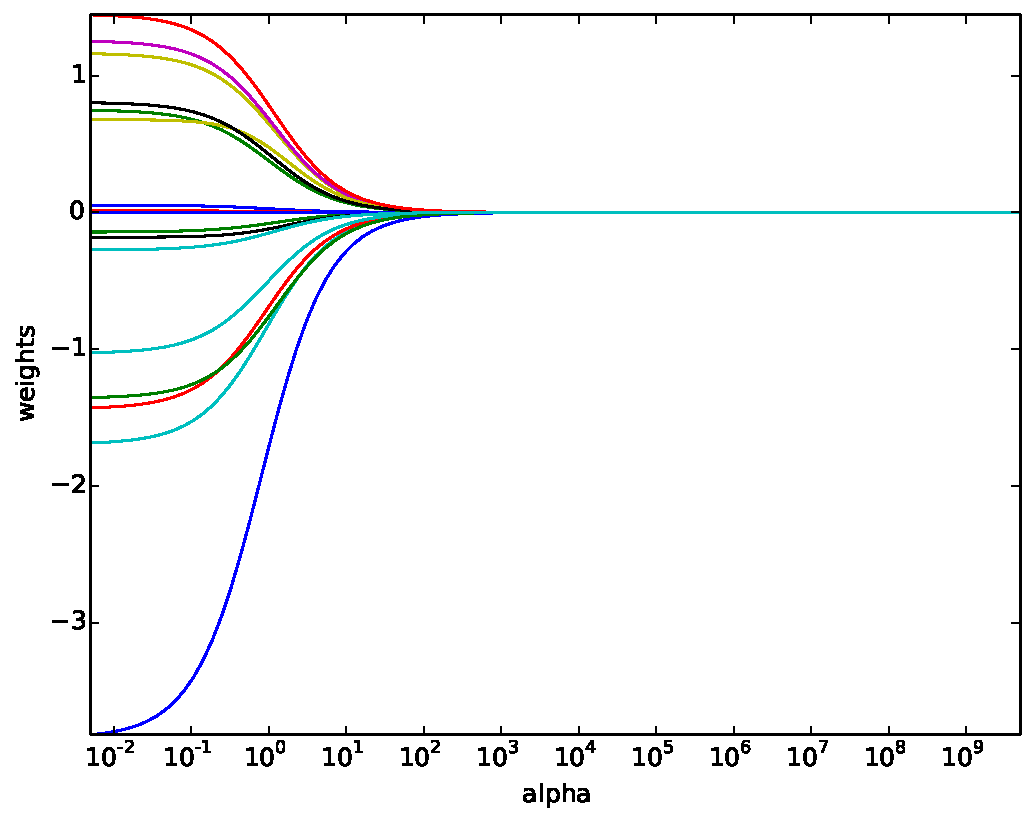
\includegraphics[width=0.5\textwidth]{wVSa.pdf}\hfill
\caption{Weights approaching $0$ as $\alpha$ increases in the example of Ridge Regression}
\label{fig:figure3}
\end{figure}

Even if Lasso has the lowest $MSE$ we see that it still \textbf{fails to meet the managers' expectations}. The reason for this performance, is that this model \textbf{does not} perform very well given that the $MSE$ is so large. The $MSE$ has the same ``units'' as the target variable and we know that \texttt{current\_satisfaction\_score} ranges from $22$ to $91$ (after cleanup), nevertheless, the $MSE$ is $208 \gg 21,91$.

\item Using the \emph{Lasso} model, we get that the $y-$intercept is approximately $7$. This means, that the baseline \texttt{current\_satisfaction\_score} is $7$. \\

The coefficients indicate the strength and type of the relationship. Firstly, we see that not all coefficients are positive which is expected based on the correlation matrix (Table 1). \\
 
 Moreover, the greater the magnitude of a coefficient, the greater the correlation between the corresponding attribute and the dependent variable. In this model we see that some of the attributes with the lowest coefficients are  \texttt{salary and average\_monthly\_hours} which is expected since as we discussed earlier these attributes have a very small correlation with \texttt{current\_satisfaction\_score}. Also, the attributes with relatively high coefficients were the departments that people are working which signifies that the attribute \texttt{department} plays a significant role in the taget variable.
 
 \item  Even if this information would be useful to have, it is true, that it would introduce sparsity in our data. Typically no more than $5-10$ employees share the same manager, therefore, including the manager of each employee would lead to a much larger number of variables used in the model. As a result our regression models would suffer from the curse of dimensionality and hence they would not perform well.
 
\end{enumerate}


 \end{homeworkProblem}


%----------------------------------------------------------------------------------------
%	PROBLEM 3
%----------------------------------------------------------------------------------------
\begin{homeworkProblem}[Problem \arabic{homeworkProblemCounter}: Classifying Employee Turnover (20 points)]
Based on market research, the product management team has identified that Xenefit's customers also want to know which employees are at risk of leaving the company (employee turnover). To develop this feature, they have collected an additional attribute that indicates if the employee left the company or not. You have been asked to perform the following tasks related to creating the employee turnover classification model.
What model do you recommend that the product management use to predict employee turnover? Explain why.

\begin{enumerate}
\item First, integrate the employee turnover information with the employee satisfaction data-set.
\item	The product management team has asked you to explain the differences between Logistic Regression, Support Vector Machines, and K-Nearest Neighbors. In particular, how do these algorithms with respect to computational complexity, performance (underfitting vs overfitting), and interpretability?
\item	Perform a set of experiments using the three learning algorithms. Which model performs the best? Explain why.
\item	What model do you recommend that the product management use to predict employee turnover? Explain why.
\end{enumerate}

\textbf{Extra credit:}\\
Create an additional model using a learning algorithm of your choice. Compare and contrast the performance of your model with the Logistic Regression, Support Vector Machine, and K-Nearest Neighbors models.

\noindent\rule{16cm}{0.9pt}
		
\large{\textbf{\underline{Answer:}}}
\begin{enumerate}
\item We see that in the file \texttt{employee\_turnover\_dataset.csv} contains the attribute \texttt{id} which is a unique identifier. Since our original dataset also contains the employees' \texttt{id} we can use this attribute to merge the two csv files. It is worth mentioning that the merging of the two files happens \textbf{after we have filtered department spelling inconsistencies} from our original csv file.

\item In terms of \textbf{complexity},  \emph{SVM and Logistic Regression} models, behave very similarly in this problem. These models minimize a convex loss functions and hence any local minimum is also guaranteed to be a global minimum as well. As far as $KNN$ is concerned, it does not minimize a loss function, yet, the computation of the ``distance'' between data points can be very expensive if many features are incorporated into the model. \\

\textbf{It has to be mentioned}, that all these models have similar complexities for relatively small number of attributes, as it is in the case of $Xenefits$. \textbf{Nevertheless}, if the management wanted to incorporate more attributes into the model then the complexities of \emph{Logistic Regression and KNN} would explode, whereas, \emph{SVM} can tackle this problem. In  \emph{SVM}, we can proceed by solving the \emph{Dual problem } instead of the \emph{Primal} and using a \emph{Kernel function} to retrieve the weights (a detailed explanation of this fact was submitted in HW2 when comparing Logistic Regression and SVM). \\

As far as \textbf{performance} is concerned, $KNN$ tend to overfit the data more easily than the other two methods. Therefore, in a $KNN$ model we should carefully decide on the parameter $K$. Similarly in an \emph{SVM} model as we increase the parameter $C$ we decrease the tolerance for misclassification but if we increase too much there is the danger of overfitting the data ($C\gg0$ is like a hard margin). Also, \emph{Logistic Regression} models can overfit but we can control the size of the coefficient of the model by introducing regularization.  \\


Finally, in terms of \textbf{interpretability} the simplest model is $KNN$ since no function minimization is involved. \emph{SVM and Logistic Regression} are more complex models which try to maximize the \emph{margin} and model the class conditional probabilities, respectively. \emph{ Logistic Regression} is always non-linear, whereas, in \emph{SVM} a non-linear Kernel function is frequently used. In the following parts we use the \textbf{Polynomial Kernel} for our \emph{SVM}  model.


\item The results for all three models were obtained through 10-fold cross validation and are summarized below (the attribute \texttt{id} is not considered in the model):
\begin{table}[H]
		\caption{Classification Models for \textbf{unnormalized} data \textbf{with} outliers}
		\centering
		\begin{tabular}{c c c}
		\hline\hline
		{} & Accuracy(\%) & F-measure   \\ [0.5ex] % inserts table %heading
		\hline
		SVM (C=1)& 76.35 & 0.671  \\  
		Logistic Regression &77.39 &0.746   \\
		KNN (K=1) & 96.71 & 0.967  \\
		ZeroR & 76.19 & 0.659 \\
		%\\ [1ex]
		\hline
		\end{tabular}\\[0.5cm]
		\label{table:nonlin}
\end{table}

In the case where we have not cleaned our dataset, we see that both \emph{SVM and Logistic Regression} perform very poorly, since they outperform the naive \emph{ZeroR} method by only $1\%$. Nevertheless, the $KNN$ method performs extremely well when comparing it to the baseline \emph{ZeroR} method. This is surprising since the data has not been normalized and hence, we would expect certain attributes  that have large magnitude (i.e. \texttt{salary}), to dominate the ``sum'' in the $KNN$ model. \\

Testing on our \textbf{clean} dataset we get the following results:
\begin{table}[H]
		\caption{Classification Models for \textbf{normalized} data \textbf{without} outliers}
		\centering
		\begin{tabular}{c c c}
		\hline\hline
		{} & Accuracy(\%) & F-measure   \\ [0.5ex] % inserts table %heading
		\hline
		SVM (C=1) & 98.32 & 0.975  \\  
		Logistic Regression &98.31 &0.975   \\
		KNN (K=1) & 98.55 & 0.986  \\
		ZeroR & 98.31 & 0.975\\
		%\\ [1ex]
		\hline
		\end{tabular}\\[0.5cm]
		\label{table:nonlin}
\end{table}

Here we see that since the baseline \emph{ZeroR} method performs so well, it is hard for the other models to significantly outperform it. Again, we observe that the $KNN$ model has the best performance in terms of Accuracy and F-measure, even though, marginally. The reason why $KNN$ performs so well must be partially attributed to the ``geometry'' of the problem. More precisely, it might be true that employees that are ``close'' (in the vector space) to each other, tend to make the same decision as to leave the company or not.

\item The model that I would propose to the company is $KNN$. The most important reason is because it seems to be performing very well in the context of this problem as we analyzed in the previous parts of this question. Moreover, since the company does not use many attributes to predict whether an employee will leave or stay in the company, the $KNN$ model is efficient.

\end{enumerate}
\end{homeworkProblem}
%----------------------------------------------------------------------------------------
%	PROBLEM 4
%----------------------------------------------------------------------------------------
\begin{homeworkProblem}[Problem \arabic{homeworkProblemCounter}: Brainstorming (10 points)]
Having been impressed by your work on the employee satisfaction and turnover models, the product management team has asked you for new ideas about how data mining can be used to improve Xenefits product offerings in the future. Apply a structured brainstorming process to generate 3-5 possible ideas for improving human resource management using data mining.\\

For each generated idea, provide a brief description of:

\begin{enumerate}
\item What human resource management problem is being addressed, e.g. improve employee engagement.
\item 	What type of data mining task is involved: classification, prediction, cluster analysis, or association analysis.
\item 	What data-sets would need to be collected for the data mining task.
\item 	How could Xenefits use the resulting model (supervised learning) or patterns (unsupervised learning) in their product offering.

\textbf{Extra credit:}\\
Implement the improvements your suggested improvements above and re-evaluate the model. Do the improvements make a difference in the model?s prediction accuracy? Explain why or why not?


\end{enumerate}



\noindent\rule{16cm}{0.9pt}
		
\large{\textbf{\underline{Answer:}}}

\begin{enumerate}
\item  \textsc{Organizational Effectiveness:}  Since we would like to assign a group on each employee (and we do not know the true label for each data point), we could use clustering which is an \textbf{unsupervised} learning technique. In this case many algorithms could be used based on our domain knowledge. If clusters tend to be globular we could use a fast \emph{K-Means} algorithm, whereas, if clusters tend to me less globular we could use \emph{DB-Scan} 

\item  \textsc{ Recruitment and availability of skilled labor:} Xenefits could apply data mining algorithms for predicting whether a university graduate would be a good fit for the company. Naturally, this falls into the binary classification problem category (supervised learning). The data that the company would have to gather for this task vary, nevertheless, some useful analytics could be the \emph{GPA, interests, specific technical skills} of the prospective employee. By using data mining, the company can look through the data quickly and can also pinpoint the best candidates with a high degree of accuracy. Recruiting skilled employees would enable Xenefits to make better the quality of its products but also explore new ideas about potential products.
	
\item  \textsc{Leadership development:} The company could attempt to predict the leadership development of any given employee from a scale of $1-100$. Xenefits could utilize this information in order to create more influential employees that could help advance further the company's products. In order extract such information, Xenefits could use prediction data mining tools such as regression. The data that would need to be available are common factors that lead to leadership enhancement such as: \emph{ability to delegate, confidence, commitment and creativity}. 

\item  \textsc{Compensation and benefits:} Instead of using standard benefits and compensation plans for all employees, Xenefits could identify what would satisfy its employees the most. Instead of relying on salary surveys or intuition, and alternative approach would be to use data to identify which types and amounts of rewards/benefits have the highest measurable impact on employee productivity. The company could use unsupervised learning clustering methods in order discover groups of employees that seek the same kind of benefits and create specialized plans. In such a way, the company could improve the quality of its products. Finally, in order to perform such an analysis, Xenefits would have to gather the preferences of each employees in terms of desirable compensations and benefits.



\end{enumerate}
\end{homeworkProblem}

\end{document}
